\section{EXPERIMENTS}
\label{sec-exp}

\subsection{Experimental Setup}
We first describe the experimental setup, including datasets, evaluation settings, comparison methods and implementation details.

\subsubsection{Datasets.}
To evaluate the effectiveness of the proposed approach, we use a large-scale production dataset from \emph{Douyin search system}.
The dataset is collected from the real online logs including 3 main search sceanrios (\ie \emph{single-column search}, \emph{double-column search}, and \emph{inner search}) and more than 20 prediction tasks.
Specifically, we collect 2-month consecutive user interaction
logs involving billions of users and hundreds of millions of documents.
Each instance incorporates over 500 features including user features, item features, sequence features and cross features.
Besides, we keep 1\% of the dataset as the evaluation data, which are excluded from the training process.
All datasets used for training and evaluation are strictly anonymized to protect user privacy.

\begin{table*}[h]
    \centering
    \caption{Performance comparison of different methods on the production dataset. The best performance and the runner-up performance are denoted in bold and underlined fonts respectively. "Improv." indicates the relative improvement ratios of the proposed approach over the best performance baselines.}
	\label{tab:results-all}
	\begin{tabular}{l c c c c c c c c c c c}
		\toprule
		\multirow{2}{*}{Method}&\multicolumn{3}{c}{Single-column Search}&&\multicolumn{3}{c}{Double-column Search}&&\multicolumn{3}{c}{Inner Search}\\
		\cmidrule{2-4}
		\cmidrule{6-8}
		\cmidrule{10-12}
		& $\text{QAUC}_{\text{Click}}$ & $\text{QAUC}_{\text{Like}}$ & $\text{QAUC}_{\text{Fav}}$ && $\text{QAUC}_{\text{Click}}$ & $\text{QAUC}_{\text{Like}}$ & $\text{QAUC}_{\text{Fav}}$ && $\text{QAUC}_{\text{Click}}$ & $\text{QAUC}_{\text{Like}}$ & $\text{QAUC}_{\text{Fav}}$\\
        \midrule
        RankMixer & 0.6389 & 0.6610 & 0.6624 && 0.6911 & 0.6621 & 0.6787 && 0.6393 & 0.6786 & 0.6621 \\
        \midrule
        SharedBottom & 0.6391 & 0.6611 & 0.6614 && 0.6929 & 0.6629 & 0.6789 && 0.6395 & 0.6794 & 0.6609\\
        MMoE & 0.6394 & 0.6614 & 0.6623 && \underline{0.6931} & \underline{0.6629} & 0.6788 && 0.6397 & 0.6793 & 0.6629 \\
        STAR & 0.6389 & 0.6611 & 0.6600 && 0.6930 & 0.6624 & 0.6784 && 0.6393 & 0.6796 & 0.6631 \\
        HMoE & \underline{0.6397} & \underline{0.6617} & 0.6623 && 0.6925 & 0.6625 & \underline{0.6790}  && 0.6401 & 0.6790 & \underline{0.6634} \\
        PEPNet & 0.6396 & 0.6609 & \underline{0.6628} && 0.6928 & 0.6625 & 0.6787  && \underline{0.6403} & \underline{0.6797} & 0.6627 \\
		\midrule
		MDL (Our) & \textbf{0.6417} & \textbf{0.6632} & \textbf{0.6656} && \textbf{0.6950} & \textbf{0.6671} & \textbf{0.6842} && \textbf{0.6419} & \textbf{0.6820} & \textbf{0.6681} \\
        Improv. & \emph{+0.31\%} & \emph{+0.23\%} & \emph{+0.42\%} && \emph{+0.27\%} & \emph{+0.63\%} & \emph{+0.77\%} && \emph{+0.25\%} & \emph{+0.34\%} & \emph{+0.71\%} \\
		\bottomrule
	\end{tabular}
\end{table*}


\subsubsection{Evaluation Settings.}
\label{subsec-evluation}
For offline evaluation, we adopt the QAUC (Query-level AUC) as the primary performance metrics, which reflects the model's ranking ability on candidates, and is widely used in personalized search system~\cite{cotrain,hyformer}.
Specifically, QAUC calculates the AUC for samples within each query and then averages the results across all queries.
It is calculated as follows:
\begin{equation}
\label{eq:qauc}
    \text{QAUC} = \frac{\sum_{i=1}^{{N}} \text{AUC}_{i}}{{N}},
\end{equation}
where $N$ is the number of distinct UID-query pairs.
To evaluate the performance across multiple scenarios and tasks, we selected three primary prediction tasks as representatives: \emph{click}, \emph{like}, and \emph{favorite}, and evaluate the performance of these prediction objectives across three different scenarios on the used production dataset.

For online evaluation, we adopt \emph{30-day user lifetime} (\ie LT30) and \emph{change query rate}.
LT30 refers to the average number of active days per user in the latest 30days, which is a important metric for DAU growth.
The \emph{change query rate} measures the probability of users manually refining a search query into a more specific one (\eg changing from "tank" to "tank300"). It is calculated as follows:
\begin{equation}
\label{eq:changeq}
    Ratio_{change} = \frac{{\tilde{N}}_\text{reform}}{{N}_\text{total}},
\end{equation}
where $\tilde{{N}}_\text{reform}$ is the number of distinct UID-query pairs with query reformulation.
This metric measures user satisfaction with the search experience, which is also widely used in personalized search system~\cite{cotrain,hyformer}.
A lower value indicates a better user experience and demonstrates a better performance of the model's predictions.

\subsubsection{Comparison Methods.}
In order to verify the effectiveness of the proposed approach, we mainly consider the following methods:

$\bullet$ \textbf{RankMixer}~\cite{RankMixer}: It adopts the token mixing and pertoken FFN strategies to capture heterogeneous feature interaction, which achieve remarkable scaling law in recommendation methods.
We use this method as a representative backbone baseline without incorporating additional multi-task or multi-scenario designs.

$\bullet$ \textbf{SharedBottom}~\cite{sharedbottom}: It adopts a classic \emph{shared-specific} framework that shares the parameters of the bottom layer and designs scenario-specific and task-specific parameter tower for each scenario and recommendation task.

$\bullet$ \textbf{MMoE}~\cite{MMoE}: It designs the shared multi-gate Mixture-of-Experts (MoE) structure to model task and scenario relationships and capture common representations from multiple scenarios and tasks.

$\bullet$ \textbf{STAR}~\cite{STAR}: It shares a centered network for all the domain and generates domain-specific network for each scenario and task.

$\bullet$ \textbf{HMoE}~\cite{HMoE}: It proposes the hybrid of implicit and explicit Mixture-of-Experts approach which learns the scenario and task relationships from feature space implicitly and label space explicitly.

$\bullet$ \textbf{PEPNet}~\cite{PEPNet}: It proposes a parameter and embedding personalized network to learn the heterogeneous relationships between multiple scenarios and multiple tasks.

Among them, except for RankMixer, all others are specifically designed for multi-scenario and multi-task recommendation models.
Therefore, in practical implementation, we integrate these methods into the RankMixer backbone, and ensure the total number of model parameters remains consistent for performance comparison.

\subsubsection{Implementation Details.}
All experiments are conducted on hundreds of GPUs in a hybrid distributed training framework that the sparse part is updated asynchronously, while the dense part is updated synchronously.
The optimizer hyperparameters are kept consistent acrossall models.
For the dense part, we used the RMSProp optimizer, while the sparse part used the Adagrad optimizer.
The batch size is set to 2048.
By adjusting the number of layers and the hidden layer dimensions of different models, we ensure that the total parameter size of all models is controlled at around 0.5B.

\subsection{Performance Comparison}
We compare the proposed approach with the aforementioned baselines on the adopted datasets, and the results are summarized in Table~\ref{tab:results-all}.
From it, we have the following observations:

Compared with Rankmixer which is a representative backbone baseline without any multi-task and multi-scenario designs, almost all the multi-scenario and multi-task baselines (SharedBottom, MMoE, STAR, HMoE and PEPNet) achieve better performance.
Because the designed shared-specific structure in these methods can better capture commonalities and characteristics between different scenarios and tasks.
Further, by comparing the proposed approach MDL with all the baselines, it is clear that MDL consistently performs better than them by a large margin on both scenarios and tasks.
It is because the proposed approach leverages tokenization to enable more comprehensive interactions among scenario, task, and feature information.

Furthermore, the proposed approach MDL demonstrates superior performance in scenarios with sparser data and tasks with lower positive sample rates.
Compared with the improvement in the single-column search, the proposed method shows even better results in the double-column search and inner search scenarios, which have sparser data.
Additionally, compared to the click task, the proposed method achieves better results in the like and favorite tasks, which have lower positive sample rates than click task.
We believe that tokenized information representation and token-level interactions can further mitigate the seesaw effect in multi-distribution learning.
During the training process, this approach allows the model to better maintain distribution modeling for relatively disadvantaged scenarios and tasks.


\begin{table}[htbp]
    \centering
    \caption{Ablation study of the proposed approach on the three scenarios ($\triangle\text{QAUC}_{\text{Click}}$).}
    \label{tab:ablation}
        \begin{tabular}{l c c c}
            \toprule
            Variants & Single & Double & Inner\\
            \midrule
            \textbf{Ablation of Task Token} \\
            \midrule
            $w/o$ task token & -0.12\% & -0.11\% & -0.09\% \\
            $w/o$ task-feature interaction & -0.04\% & -0.05\% & 0.03\% \\
            \midrule
            \textbf{Ablation of Scenario Token} \\
            \midrule
            $w/o$ scenario token & -0.17\% & -0.16\% & -0.15\% \\
            $w/o$ global scenario token & -0.04\% & -0.06\% & -0.05\% \\
            $w/o$ scenario-feature intraction & -0.05\% & -0.04\% & -0.05\% \\
            \bottomrule
        \end{tabular}
\end{table}

\subsection{Ablation Study}
In this part, we continue to analyze how each of the proposed techniques or components affects the final performance.
We prepare five variants of the proposed approach MDL for comparisons, including:

$\bullet$ $w/o$ task token: without all task tokens from the input, and leverage task-tower for multi-task learning.

$\bullet$ $w/o$ task-feature interaction: replace domain-aware attention on task tokens with interaction in Rankmixer.

$\bullet$ $w/o$ scenario token: without all scenario tokens from the input, and leverage scenario-tower for multi-scenario learning.

$\bullet$ $w/o$ global scenario token: without the global scenario token from the input.

$\bullet$ $w/o$ scenario-feature interaction: replace domain-aware attention on scenario tokens with interaction in Rankmixer.

The experimental results of the MDL variants are reported in Table~\ref{tab:ablation}.
From it, we can observe that removing each of the components leads to the performance decrease.
The variant $w/o$ task token and $w/o$ scenario token indicate the importance of tokenization of scenario information and task information.
The variant $w/o$ global scenario token shows the importance of the global token.
The variants $w/o$ task-feautre interaction and $w/o$ scenario-feature interaction indicate the effectiveness of the elaborated interaction mechanisms among these tokens.

\subsection{Further Analysis}
In this section, we further perform a series of detailed analyses on
the proposed MDL to confirm its effectiveness.

\begin{figure}[t]
    \centering
    \subfigure[QAUC scaling with model params.]{
        \centering
        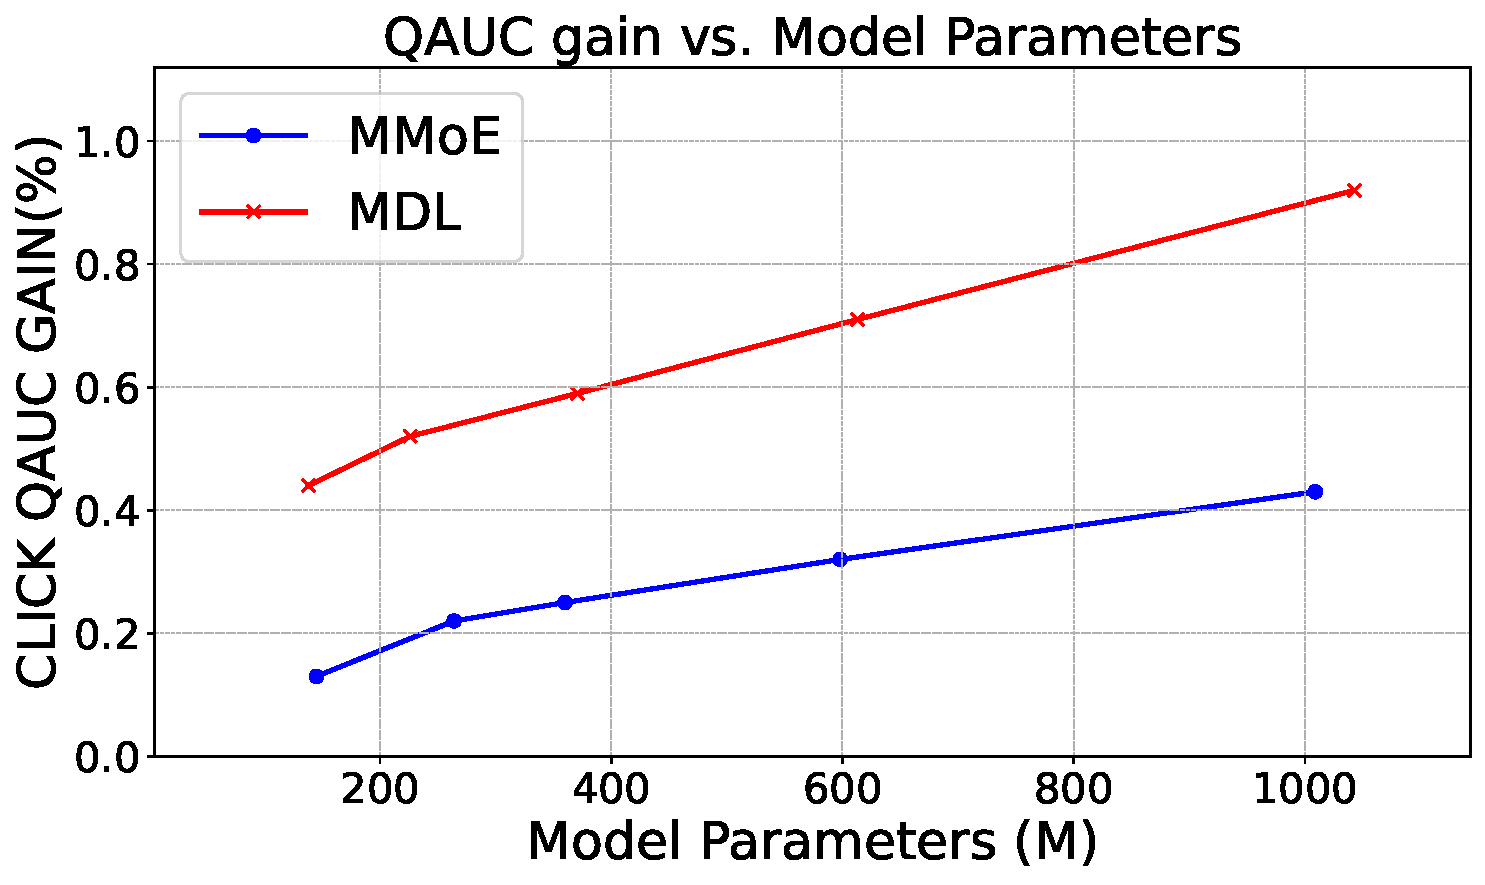
\includegraphics[width=0.225\textwidth]{assets/exp-sl-params2.pdf}
    }
    \subfigure[QAUC scaling with model FLOPs.]{
        \centering
        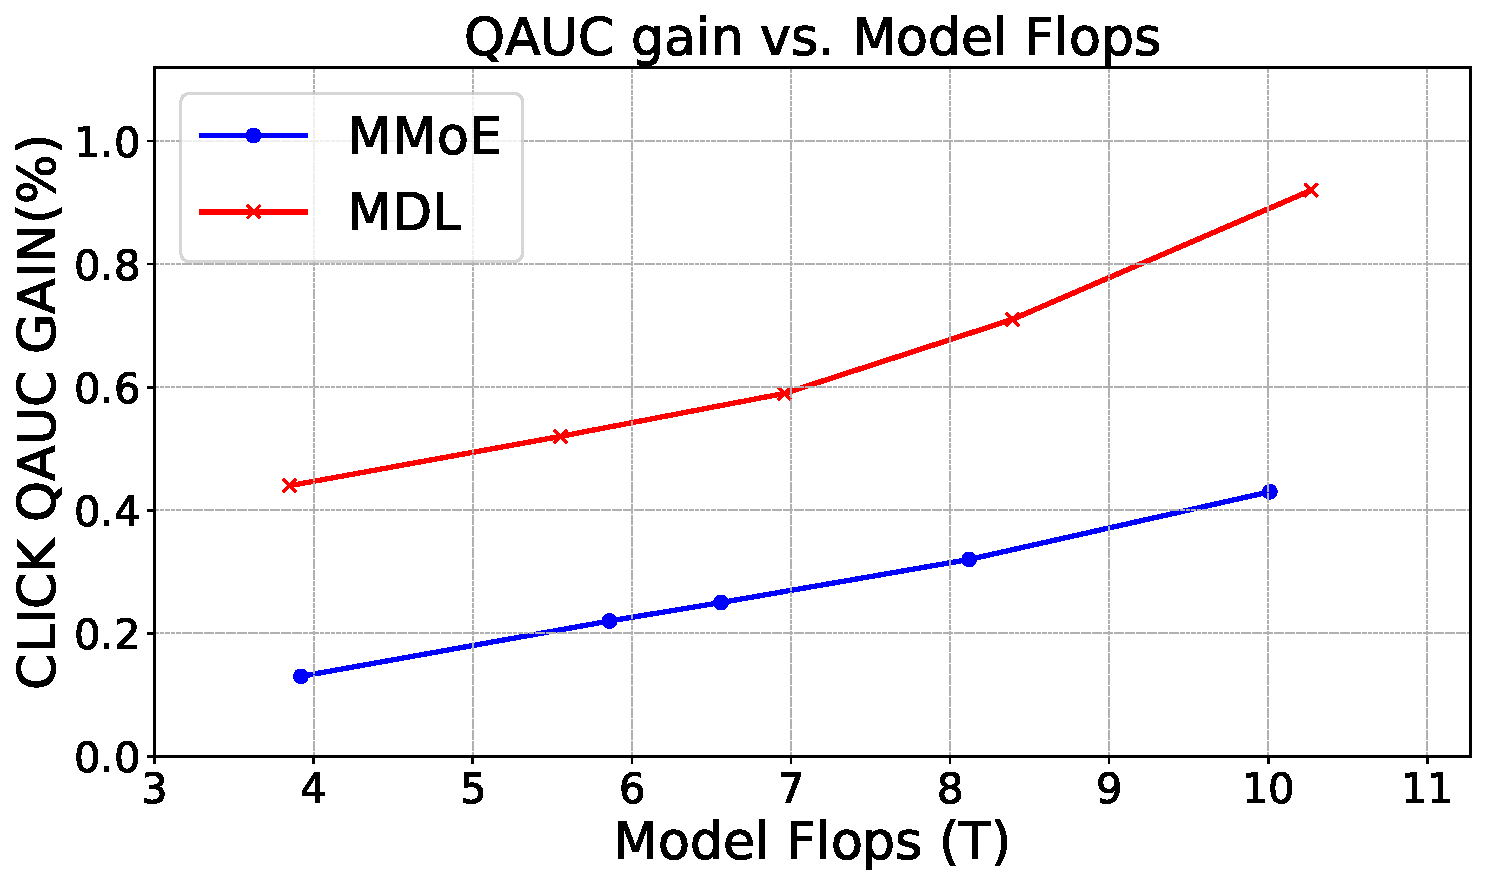
\includegraphics[width=0.225\textwidth]{assets/exp-sl-flops2.pdf}
    }
\caption{Scaling laws between click QAUC gain on single-column search scenario and model parameters/FLOPs of different models.}
\label{fig:exp-sl}
\end{figure}


\subsubsection{Performance Comparison \wrt Scaling Laws}
In this part, we examine how the proposed approach performs \wrt the model parameters and model FLOPs.
For this purpose, we adjust the model's hidden representations $d$ and the number of layers $L$ to control the model's parameter size and FLOPs.
Then we compare the performance of MDL and the representive baseline MMoE on these settings, and report the results in Figure~\ref{fig:exp-sl}.
From this, we can find that the performance of MDL is consistently better than MMoE.
Meanwhile, as the model params and FLOPs increase, the performance gain brought by MDL increases.
Compared with previous multi-scenario and multi-task recommendation methods, the proposed approach can better leverage the model parameters for multi-distribution learning through the token-level interaction layer-by-layer, fully harvesting the benefits of the scaling law.


\begin{figure}[t]
    \centering
    \subfigure[Click task on layer1.]{
        \centering
        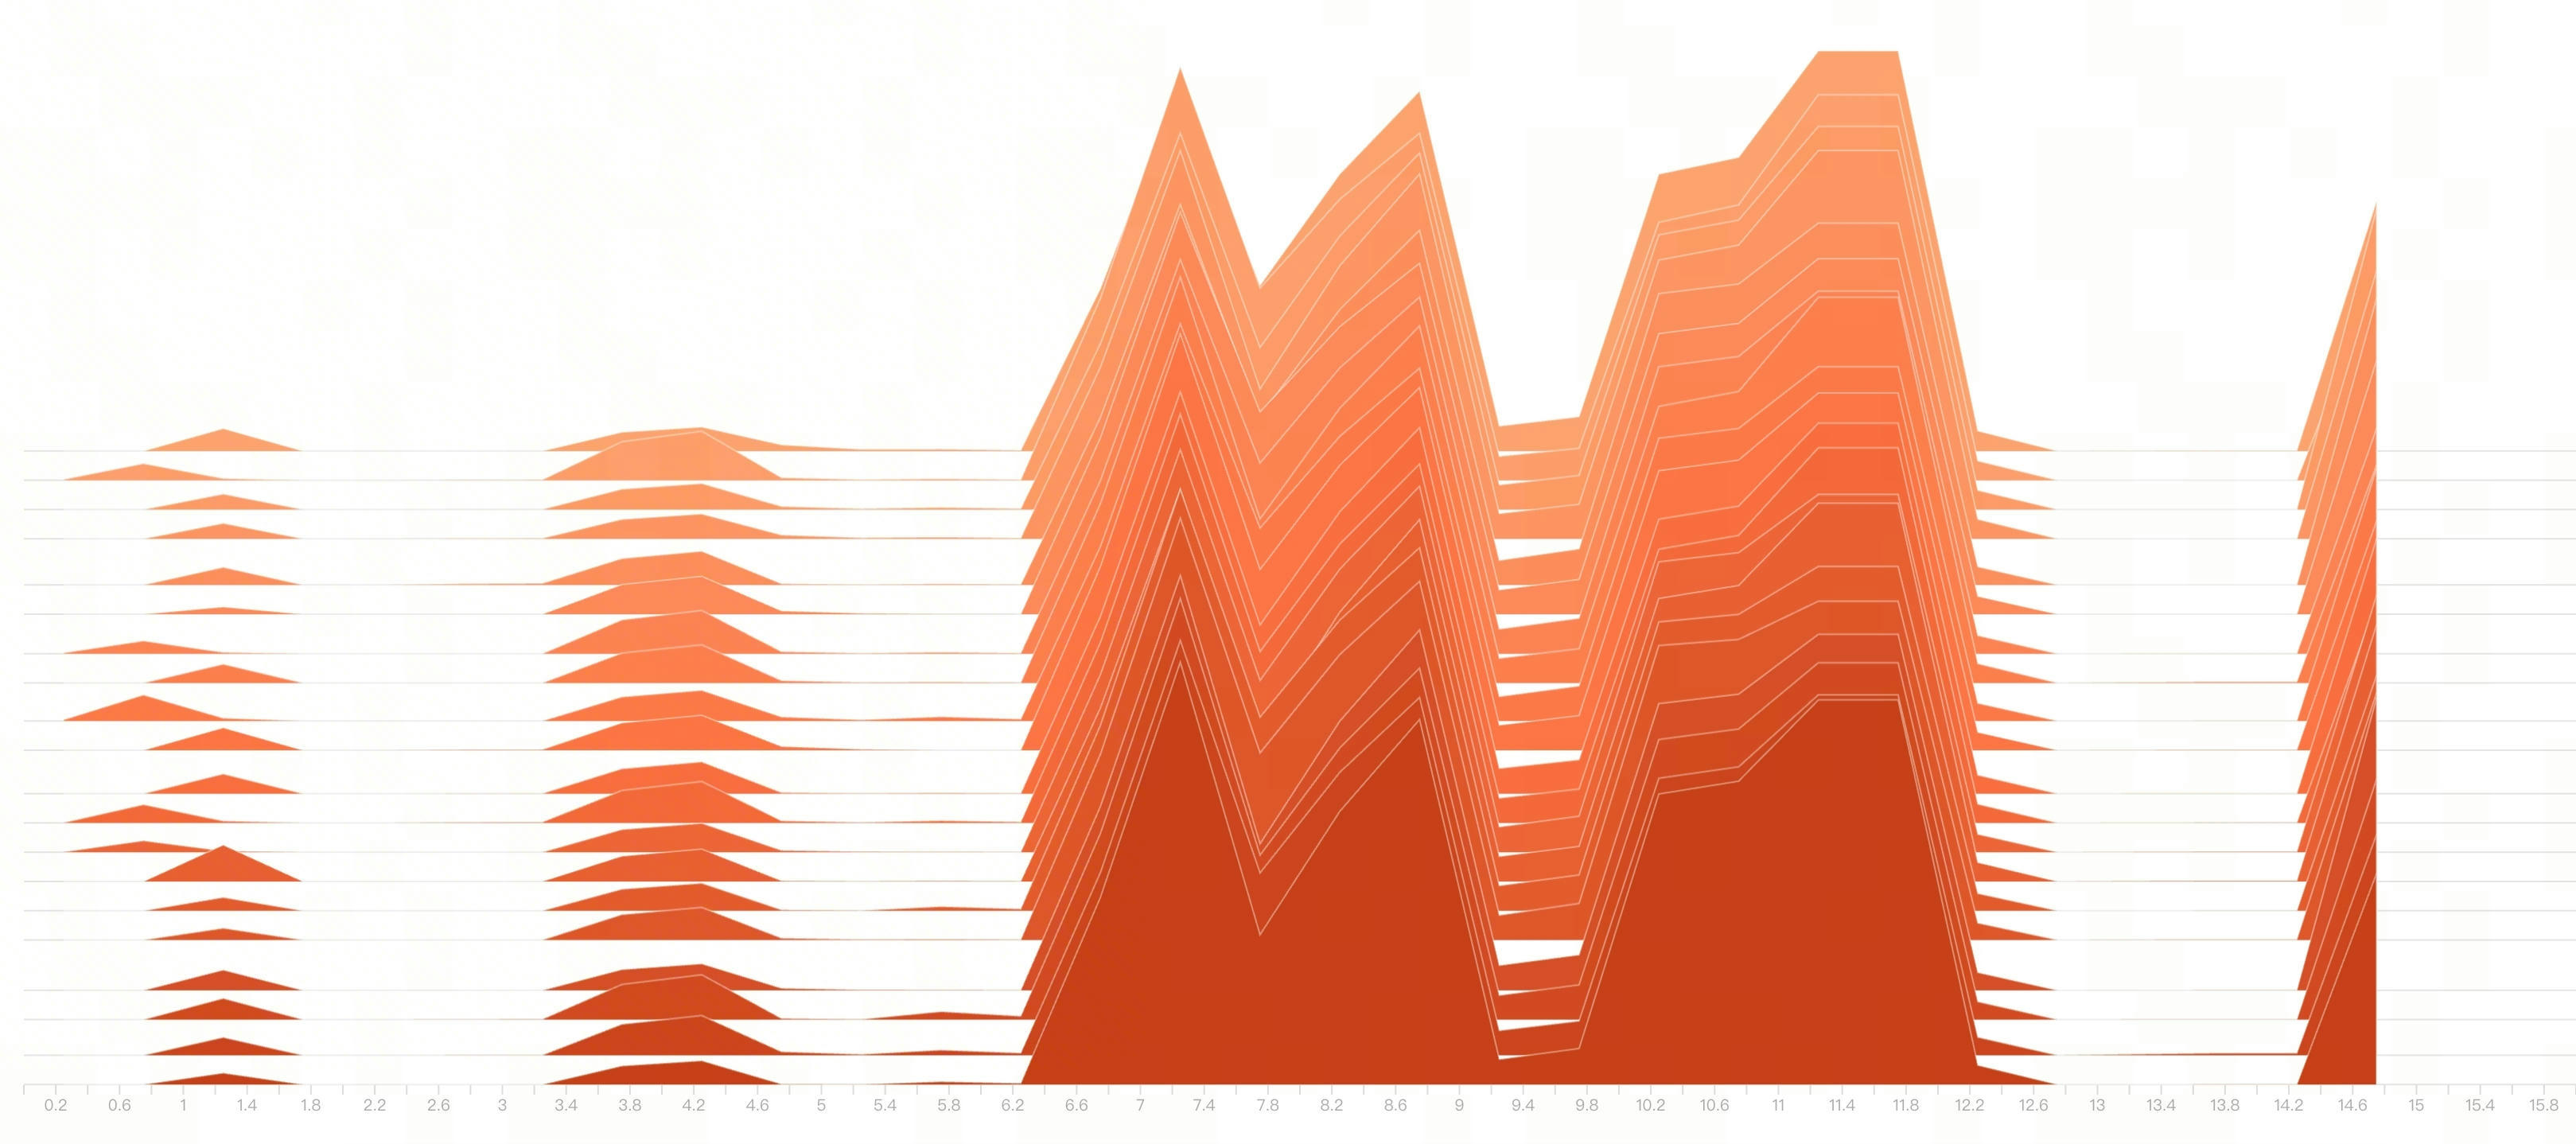
\includegraphics[width=0.225\textwidth]{assets/click_layer1.jpg}
    }
    \subfigure[Click task on layer2.]{
        \centering
        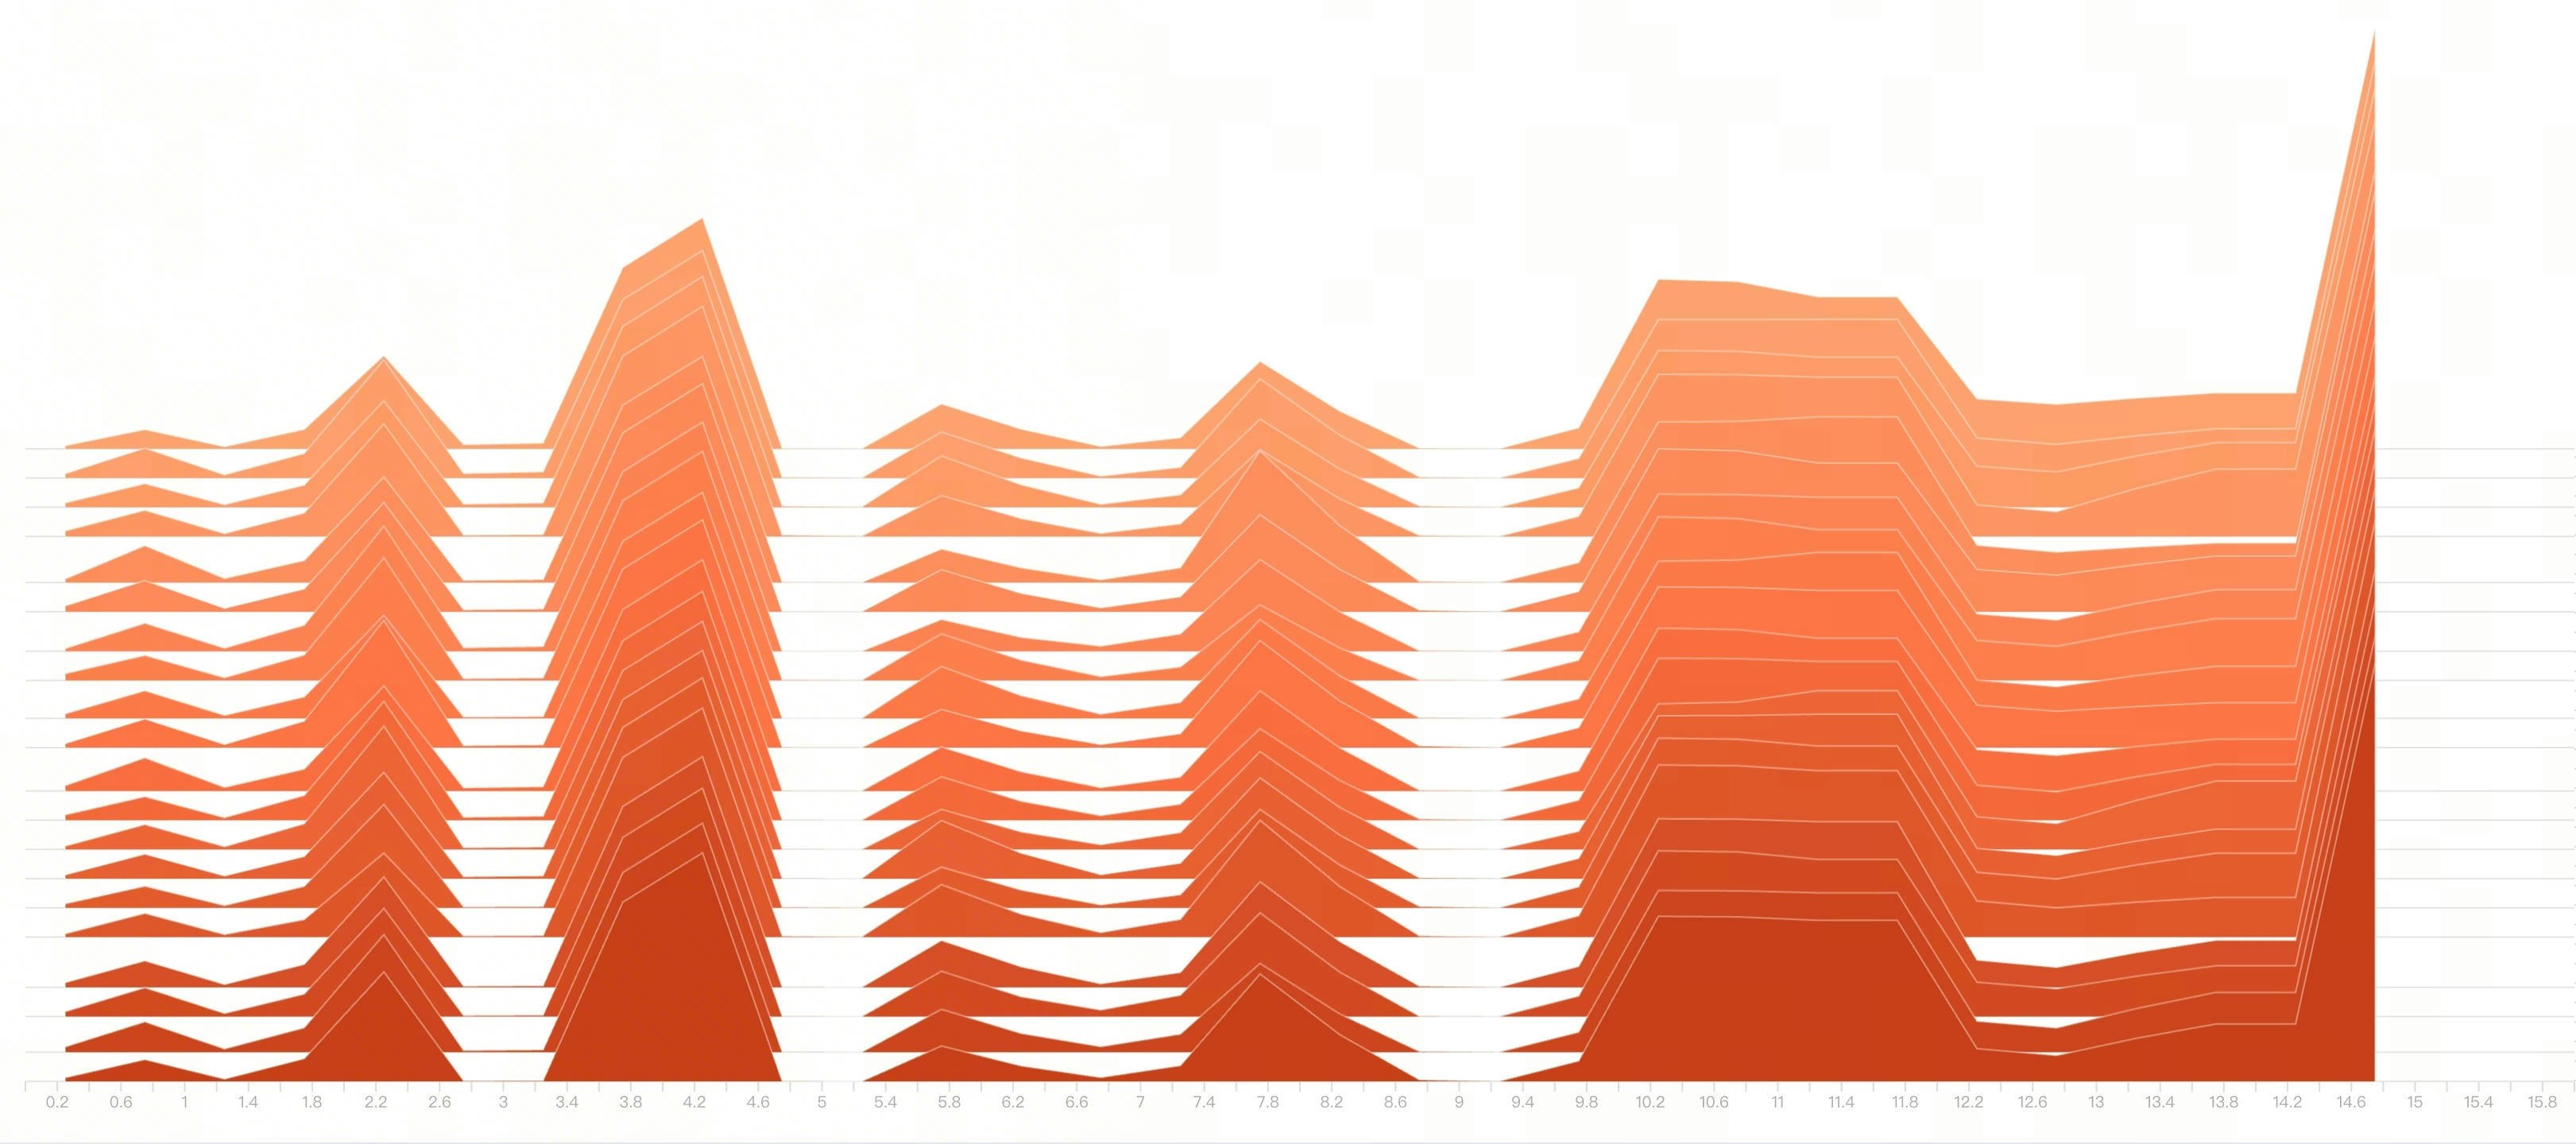
\includegraphics[width=0.225\textwidth]{assets/click_layer2.jpg}
    }
    \subfigure[Like task on layer1.]{
        \centering
        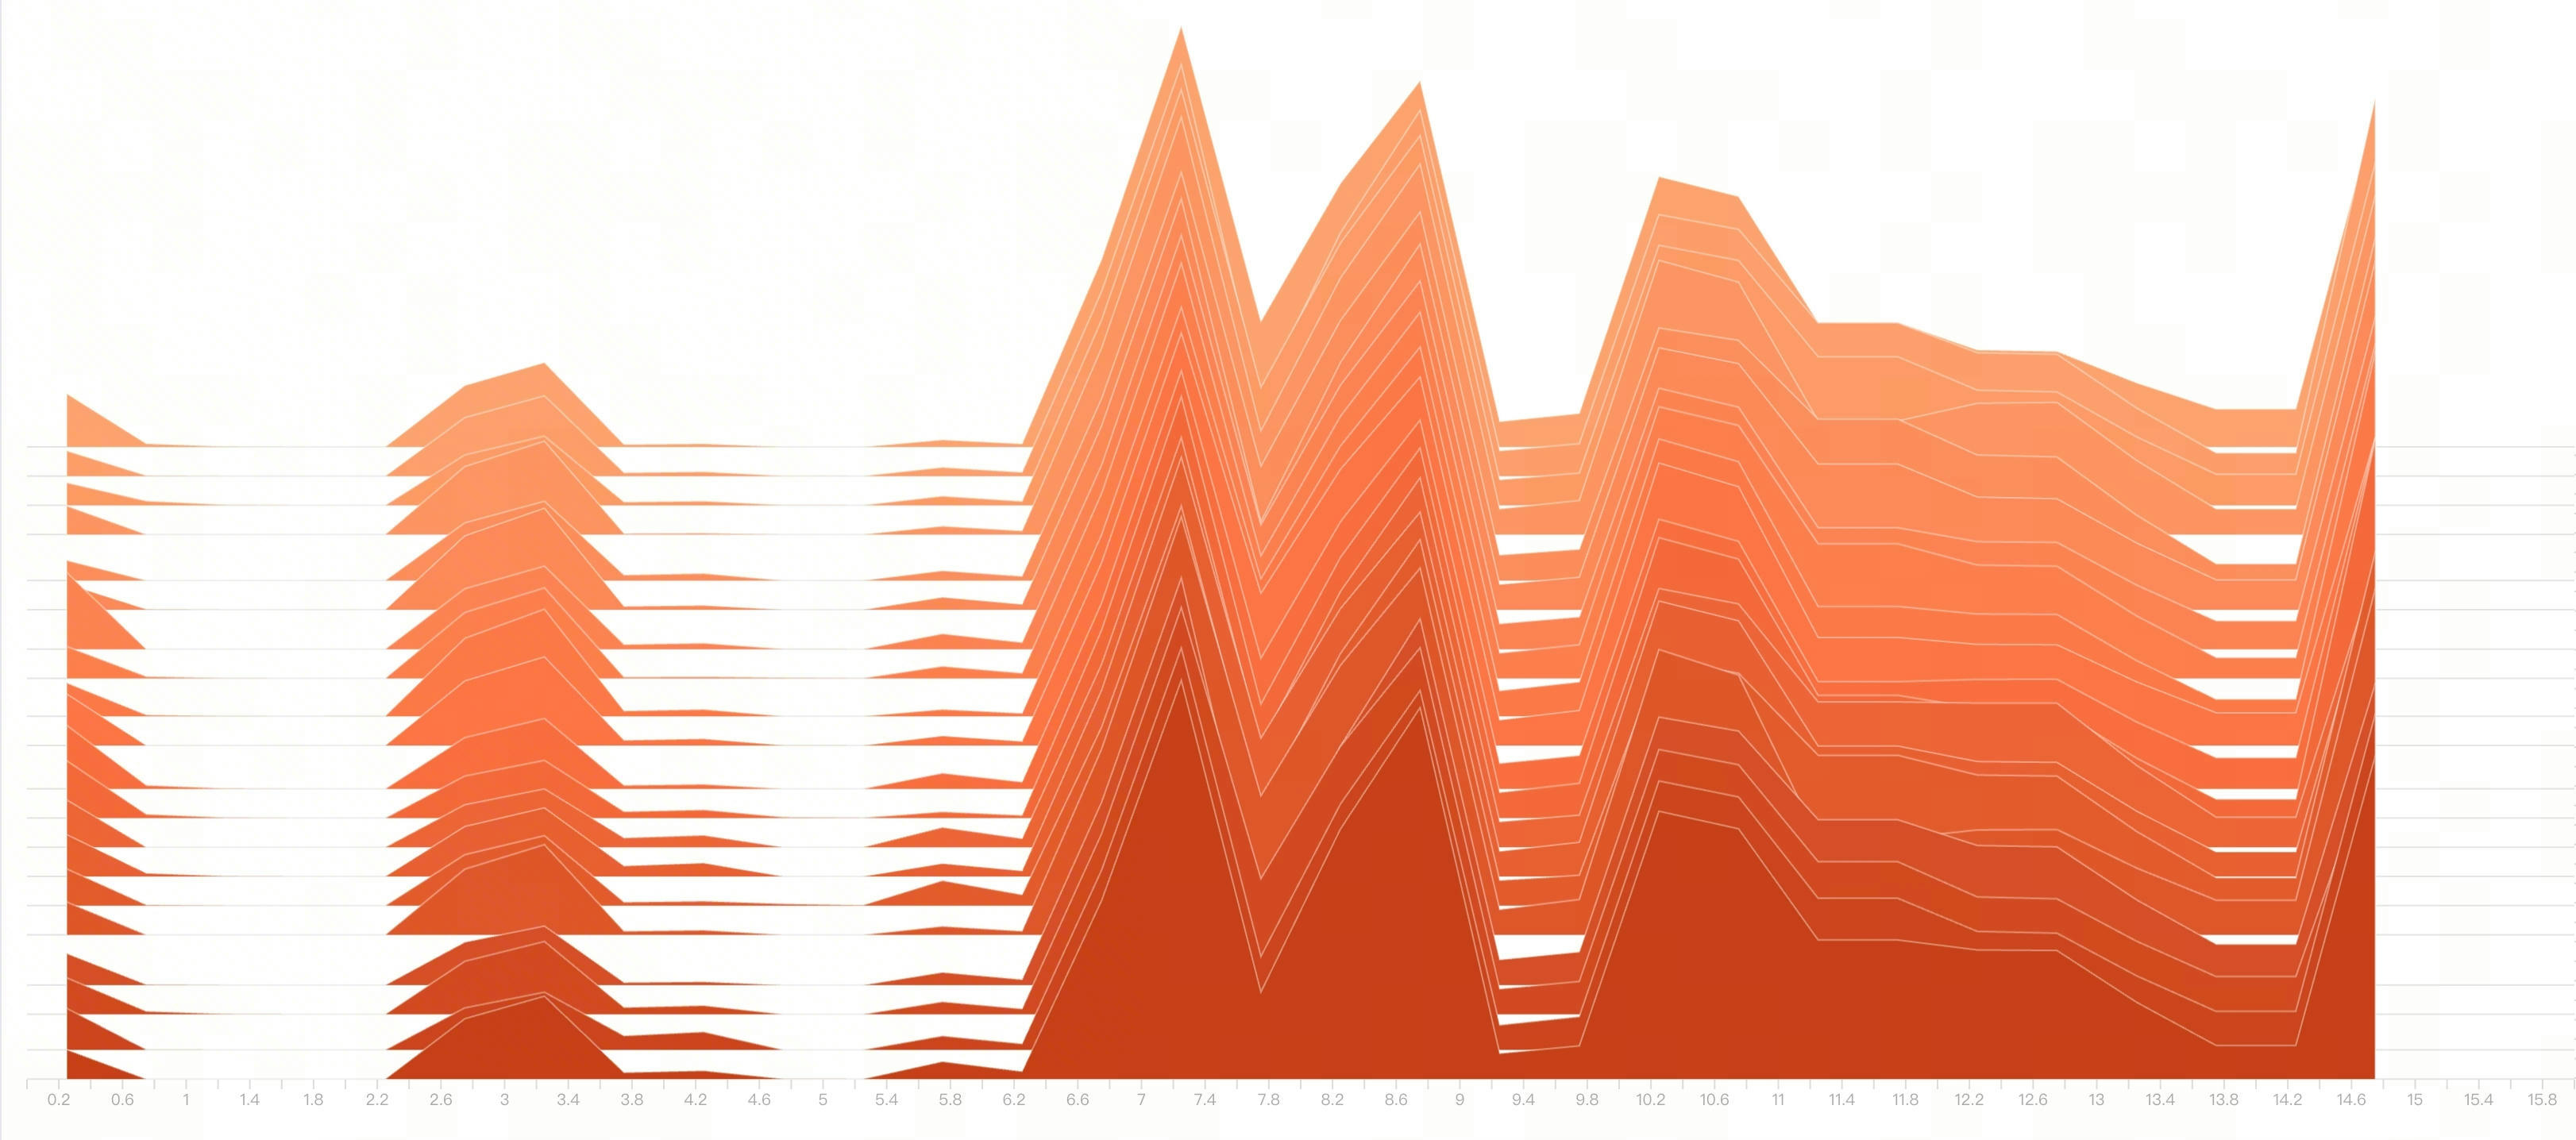
\includegraphics[width=0.225\textwidth]{assets/like_layer1.jpg}
    }
    \subfigure[Like task on layer2.]{
        \centering
        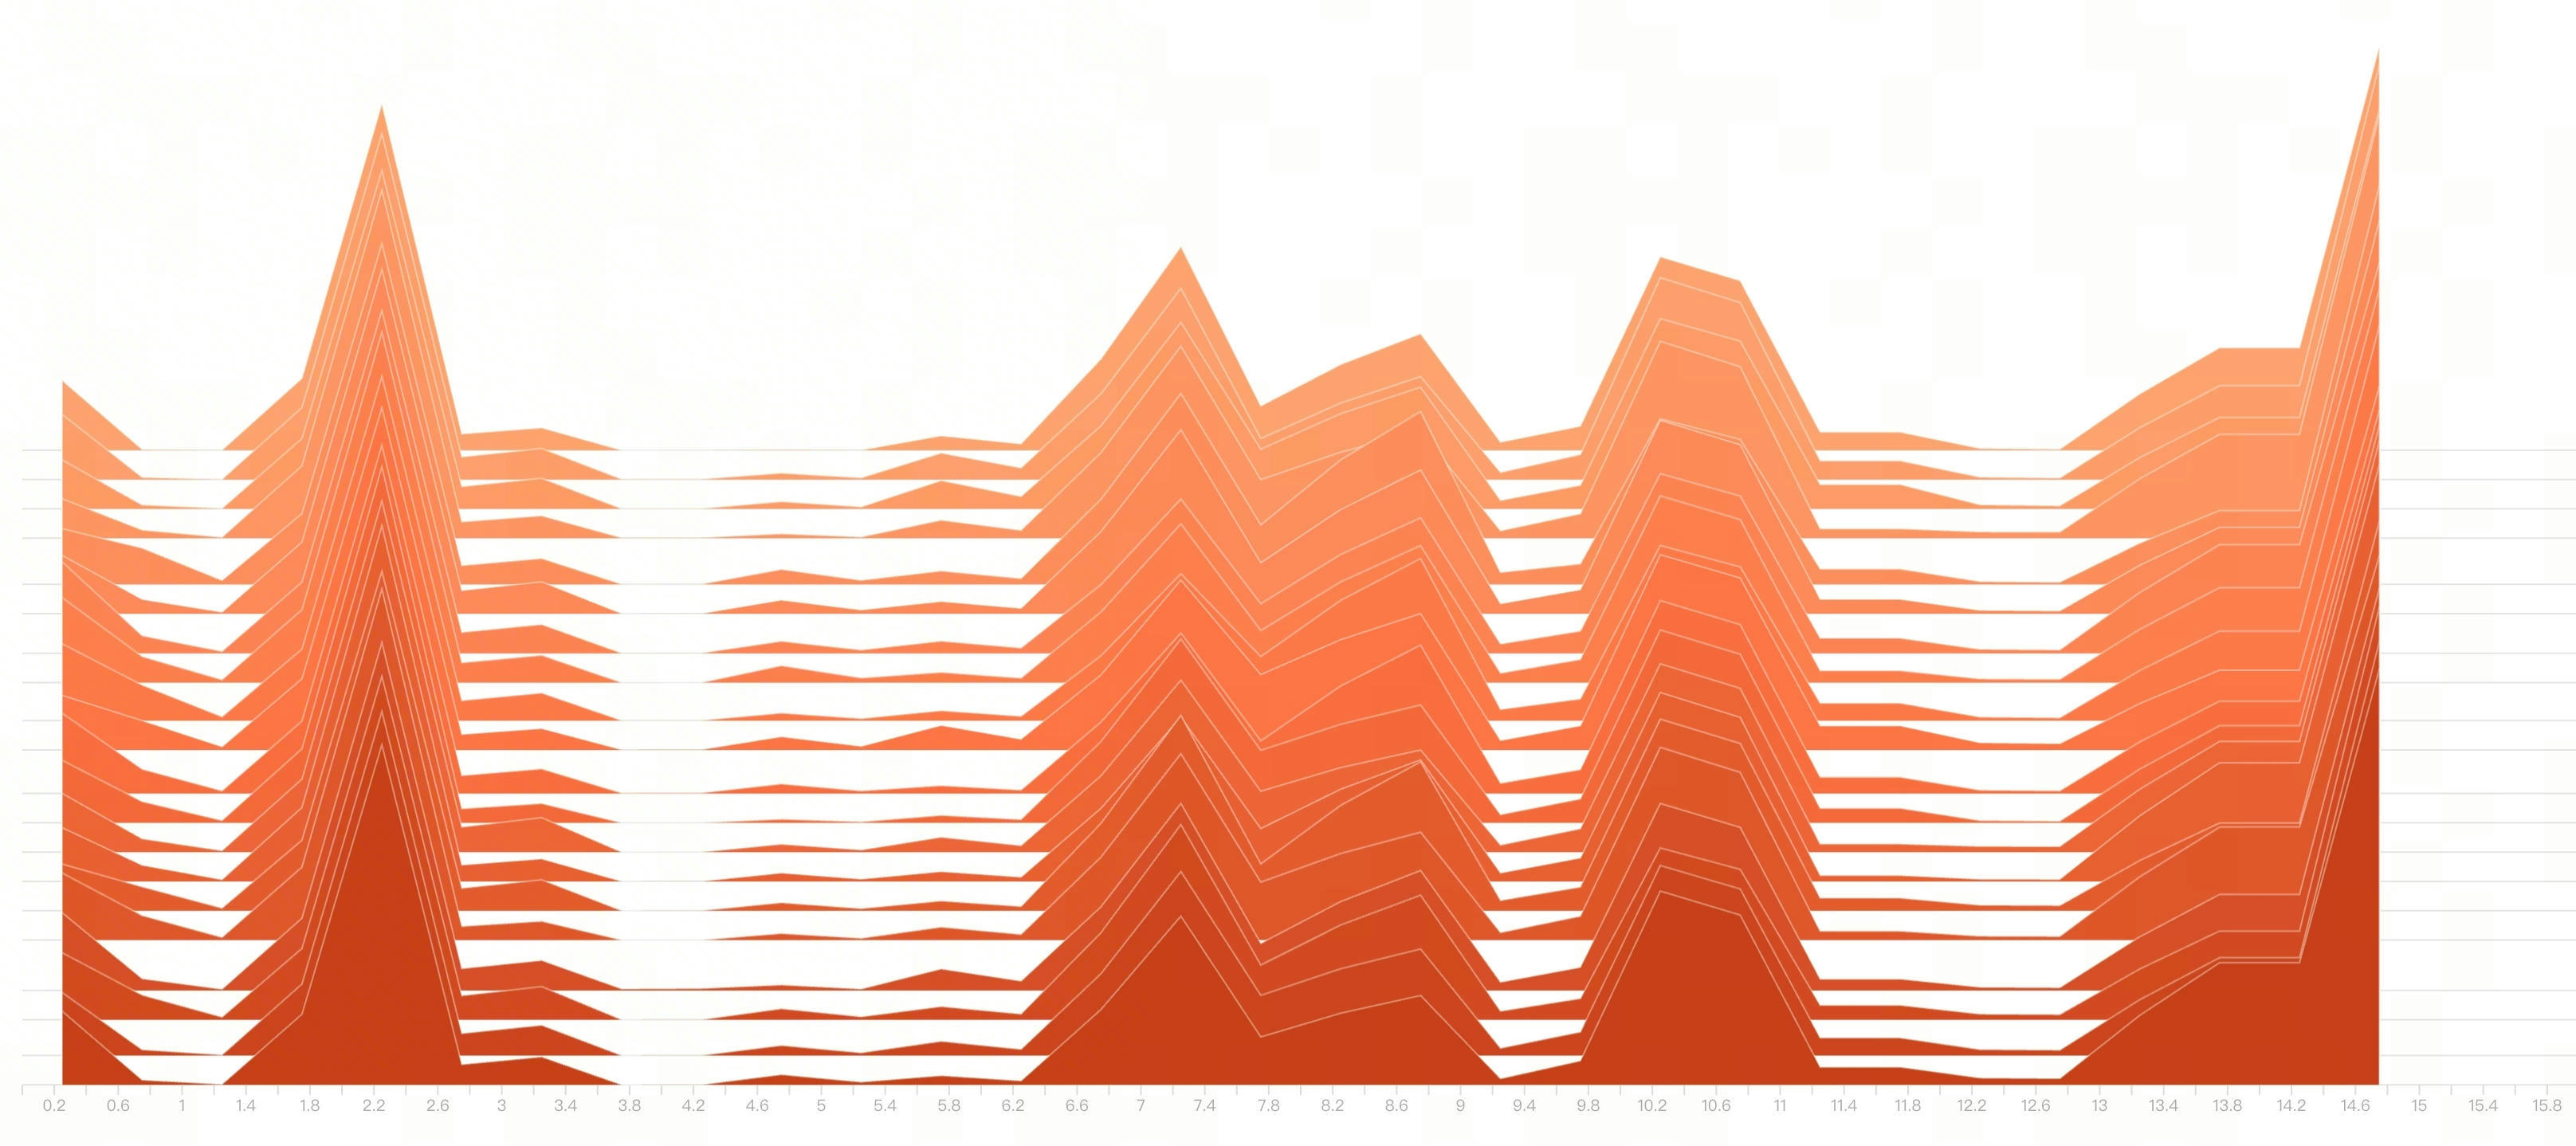
\includegraphics[width=0.225\textwidth]{assets/like_layer2.jpg}
    }
\caption{Attention distribution between task tokens and feature tokens on different layers. The x-axis represents the index of feature tokens and y-axis represents the average attention weights belong to the corresponding feature token.}
\label{fig:exp-vis1}
\end{figure}

\begin{figure}[t]
    \centering
    \subfigure[Single-column search scenario.]{
        \centering
        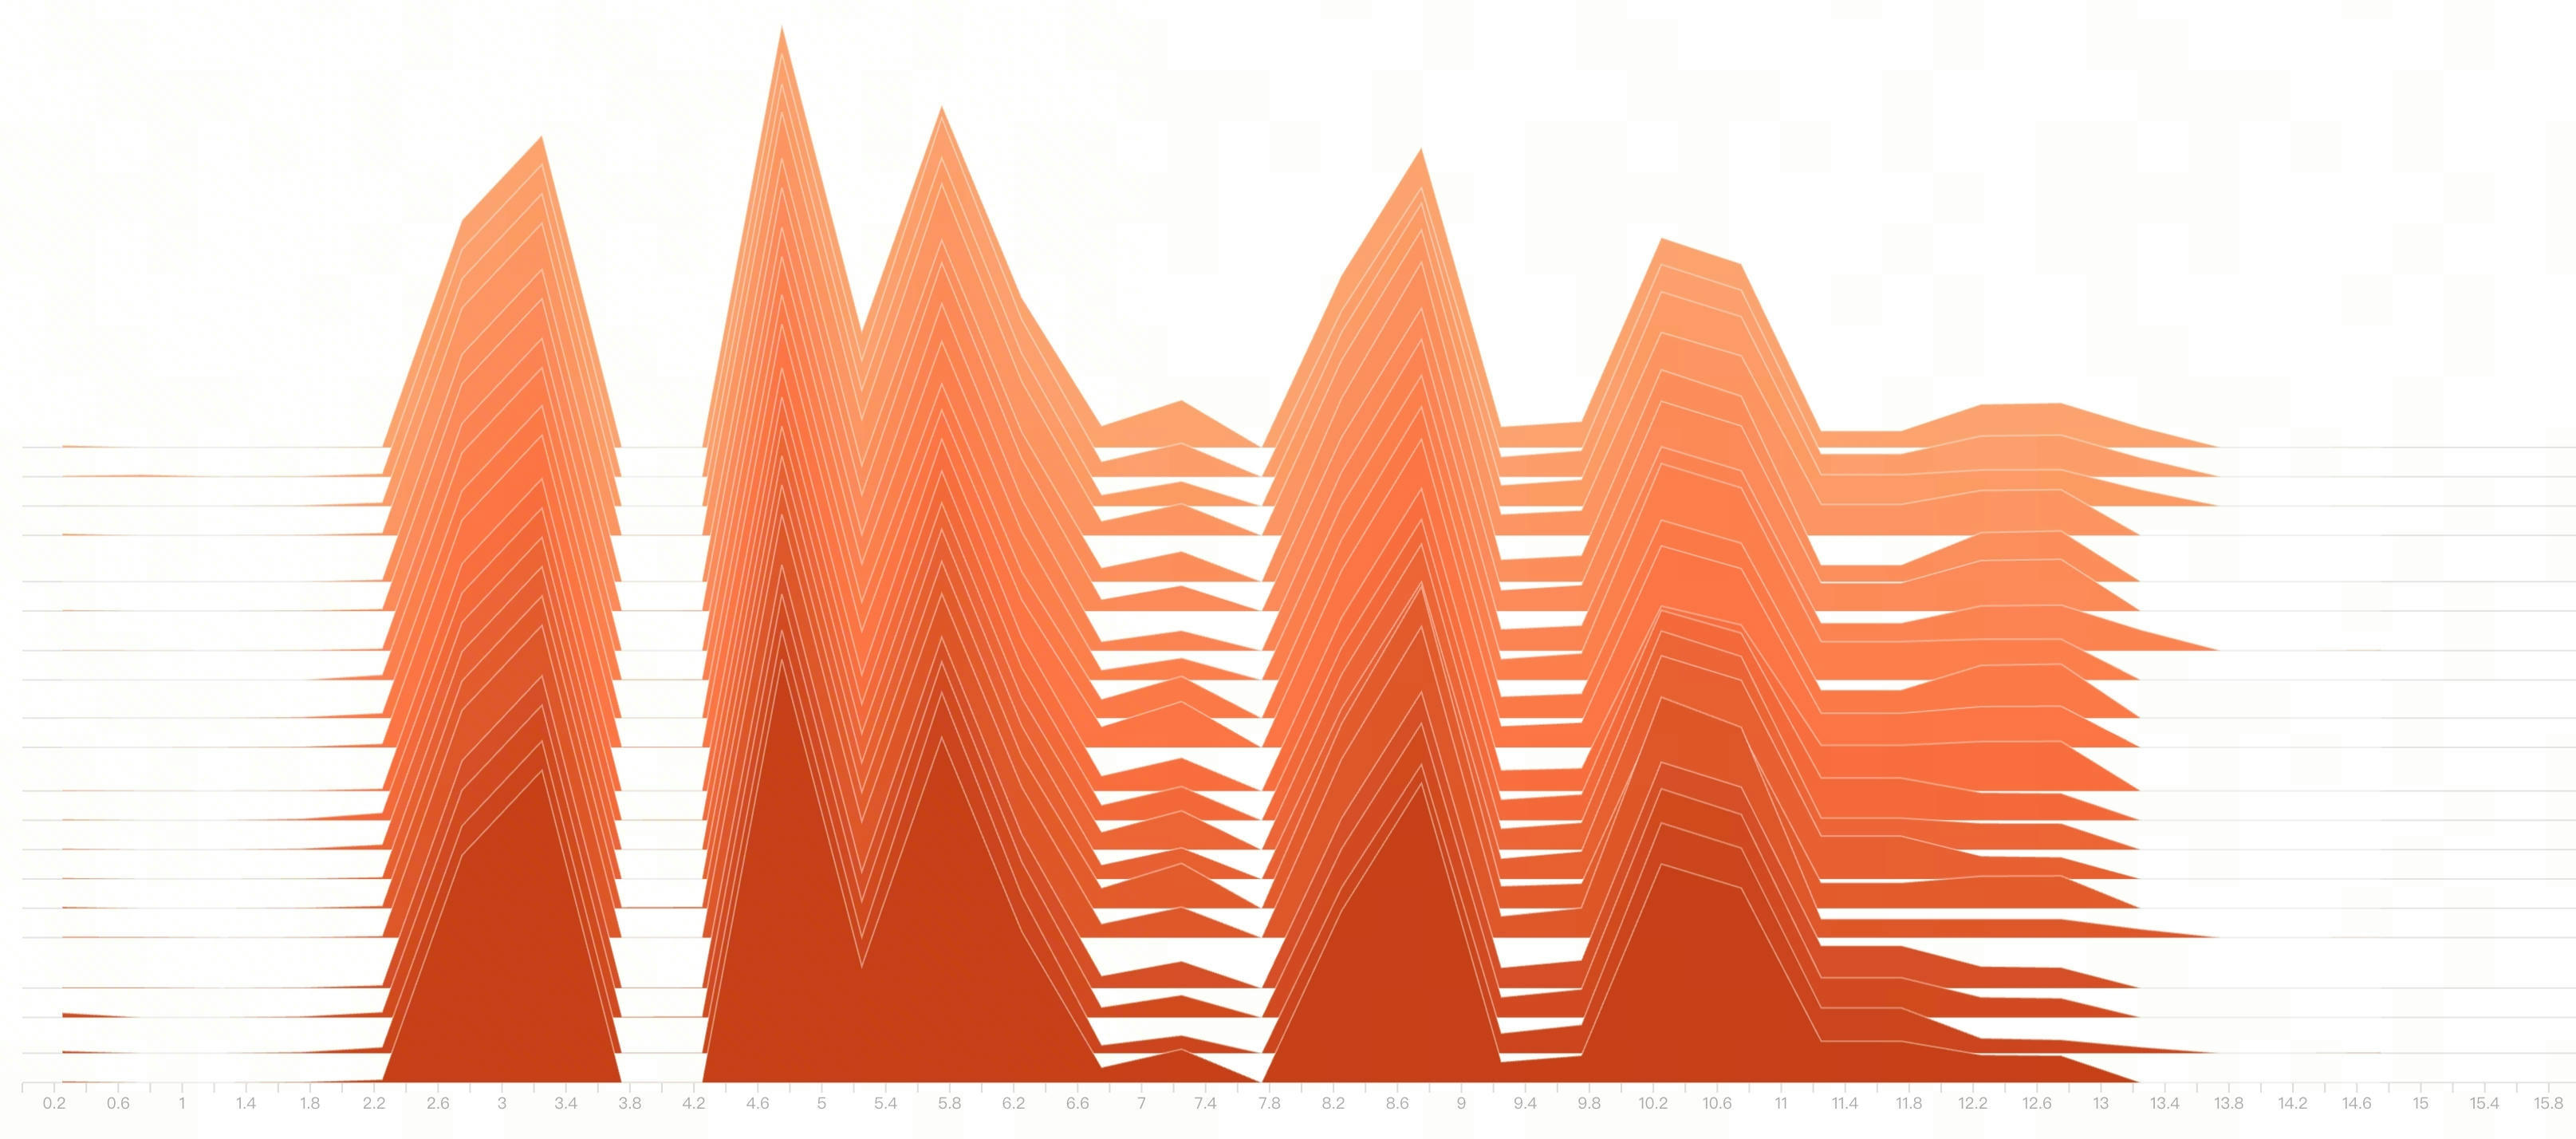
\includegraphics[width=0.225\textwidth]{assets/single_layer2.jpg}
    }
    \subfigure[Double-column search scenario.]{
        \centering
        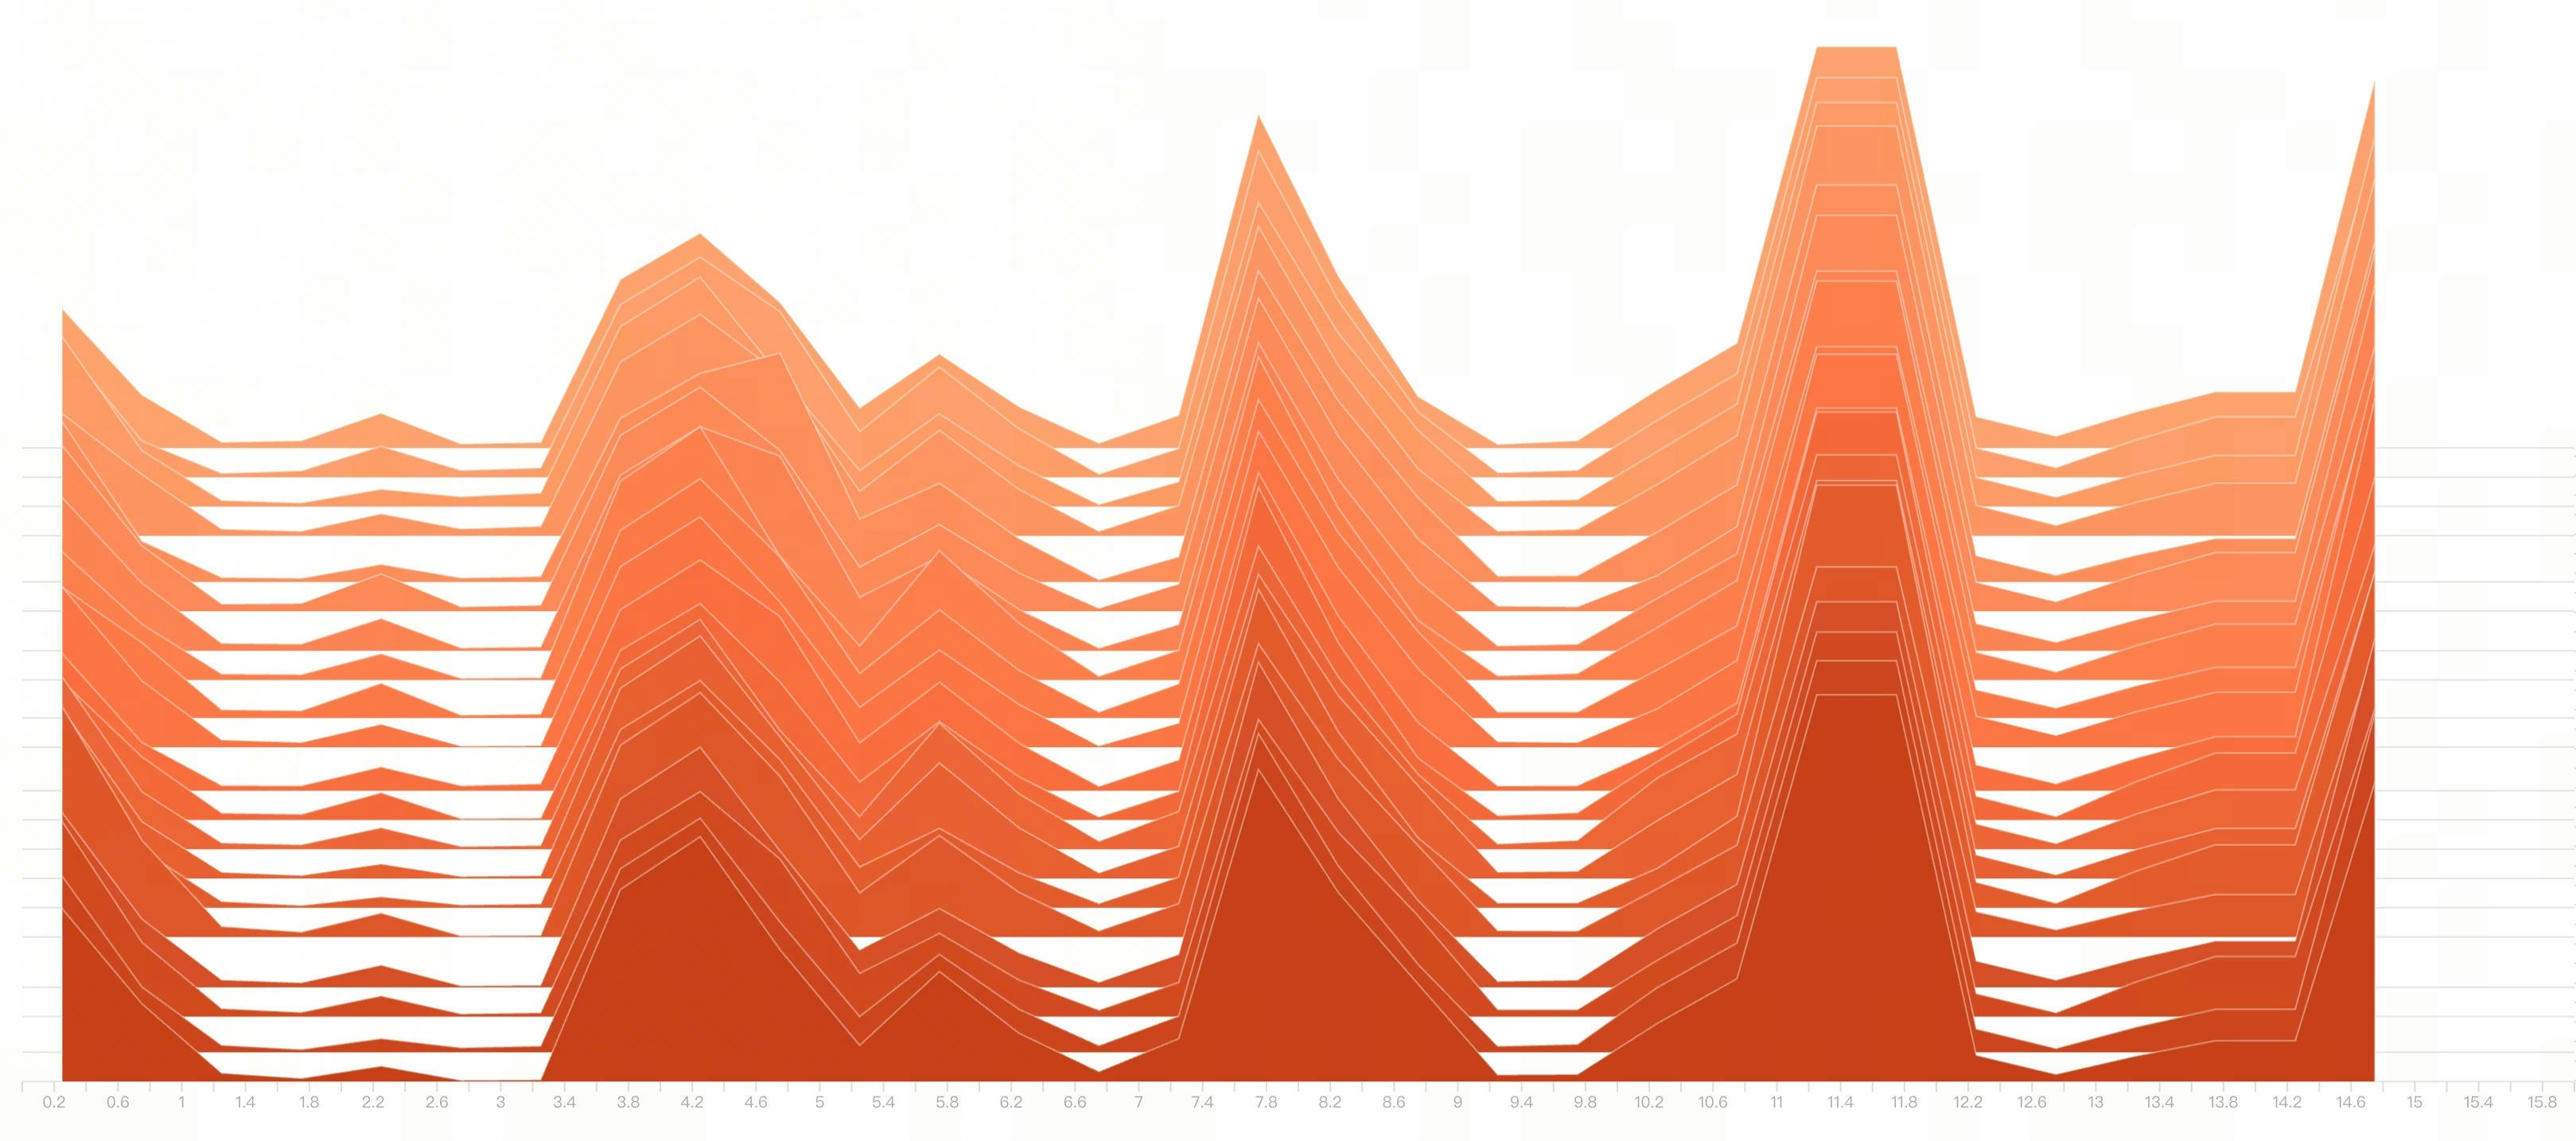
\includegraphics[width=0.225\textwidth]{assets/double_layer2.jpg}
    }
\caption{Attention distribution between scenario tokens and feature tokens. The x-axis represents the index of feature tokens and y-axis represents the average attention weights belong to the corresponding feature token.}
\label{fig:exp-vis2}
\end{figure}

\subsubsection{Visualizing the Attention Score}
A key component of the proposed approach MDL is the interaction between feature tokens and scenario/taks tokens.
Through the \emph{domain-aware attention}, the task tokens and scenario tokens can adaptively and selectively aggregate the rich information from feature tokens based on their own data characteristics for achieving differentiated modeling for multi-scenario and multi-task learning.
To better prove and understand the benefits brought by the domain-aware attention, we visualize the learned attention distributtion from different task tokens and scenario tokens in Figure~\ref{fig:exp-vis1} and Figure~\ref{fig:exp-vis2}.

From Figure~\ref{fig:exp-vis1}, we can observe that within the same layer, the attention distribution between different task tokens and feature tokens is different.
This indicates that different task tokens have learned distinct information for their respective distributions, thereby modeling the differences between tasks.
Moreover, for the attention distribution between the same task token and feature tokens, the attention distribution varies across different layers.
This indicates that as information interaction progresses layer by layer, task tokens can dynamically capture these changes and adaptively aggregate the corresponding information.
Similarly, from Figure~\ref{fig:exp-vis2}, we can observe that the the attention distribution between different scenario tokens and feature tokens is also different.


\begin{table}[t]
    \centering
    \caption{Results of online A/B tests on Douyin Search (relative improvements).}
    \label{tab:online}
        \begin{tabular}{ccc}
            \toprule
            Scenario & Change Query Rate & LT30 \\
            \midrule
            ALL & -0.3267\% & +0.0626\%  \\
            \cmidrule{1-3}
            Single-column Search & -0.2678\% & +0.0520\%  \\
            Double-column Search & -0.5079\% & +0.0674\%  \\
            Inner Search & -0.5492\% & +0.0630\%  \\
            \bottomrule
        \end{tabular}
\end{table}

\subsection{Online Experiments}
\label{exp:online}
To further verify the effectiveness of the proposed approach \modelname, we conducted an online A/B test on Douyin Search for one month.
The online base model is based on RankMixer~\cite{RankMixer}, with multi-scenario and multi-task learning implemented via MMoE~\cite{MMoE}.
The core online metrics include change query rate and LT30, as introduced in Section~\ref{subsec-evluation}.
Table~\ref{tab:online} reports the relative improvements in the different scenarios and the overall performance.
The proposed method yielded +0.0626\% improvement in LT30 and -0.3267\% reduction in change query rate.
As for each scenario, it also achieved significant improvements on the core metrics.


